\documentclass{article}

\usepackage[utf8]{inputenc}
\usepackage[T1]{fontenc}
\usepackage[francais]{babel}
\usepackage[top = 1.5cm, left = 1.5cm, right =1.5cm, bottom = 1.5cm]{geometry}
\usepackage[pdfborder ={0 0 0}]{hyperref}
\usepackage{graphicx}
\usepackage{xcolor}
\usepackage{multicol}
\usepackage{lscape}
\usepackage{datatool}
\usepackage{pdfpages}
\usepackage{rotating}

\begin{document}

\begin{titlepage}
\begin{figure}
\end{figure}

\title{\vspace{1cm}{\Huge \bf{Management Project} } \\ \vspace{2cm} \bf{Mold \& Co in China} \vspace{1cm} \\
}
\begin{figure}
\begin{center}
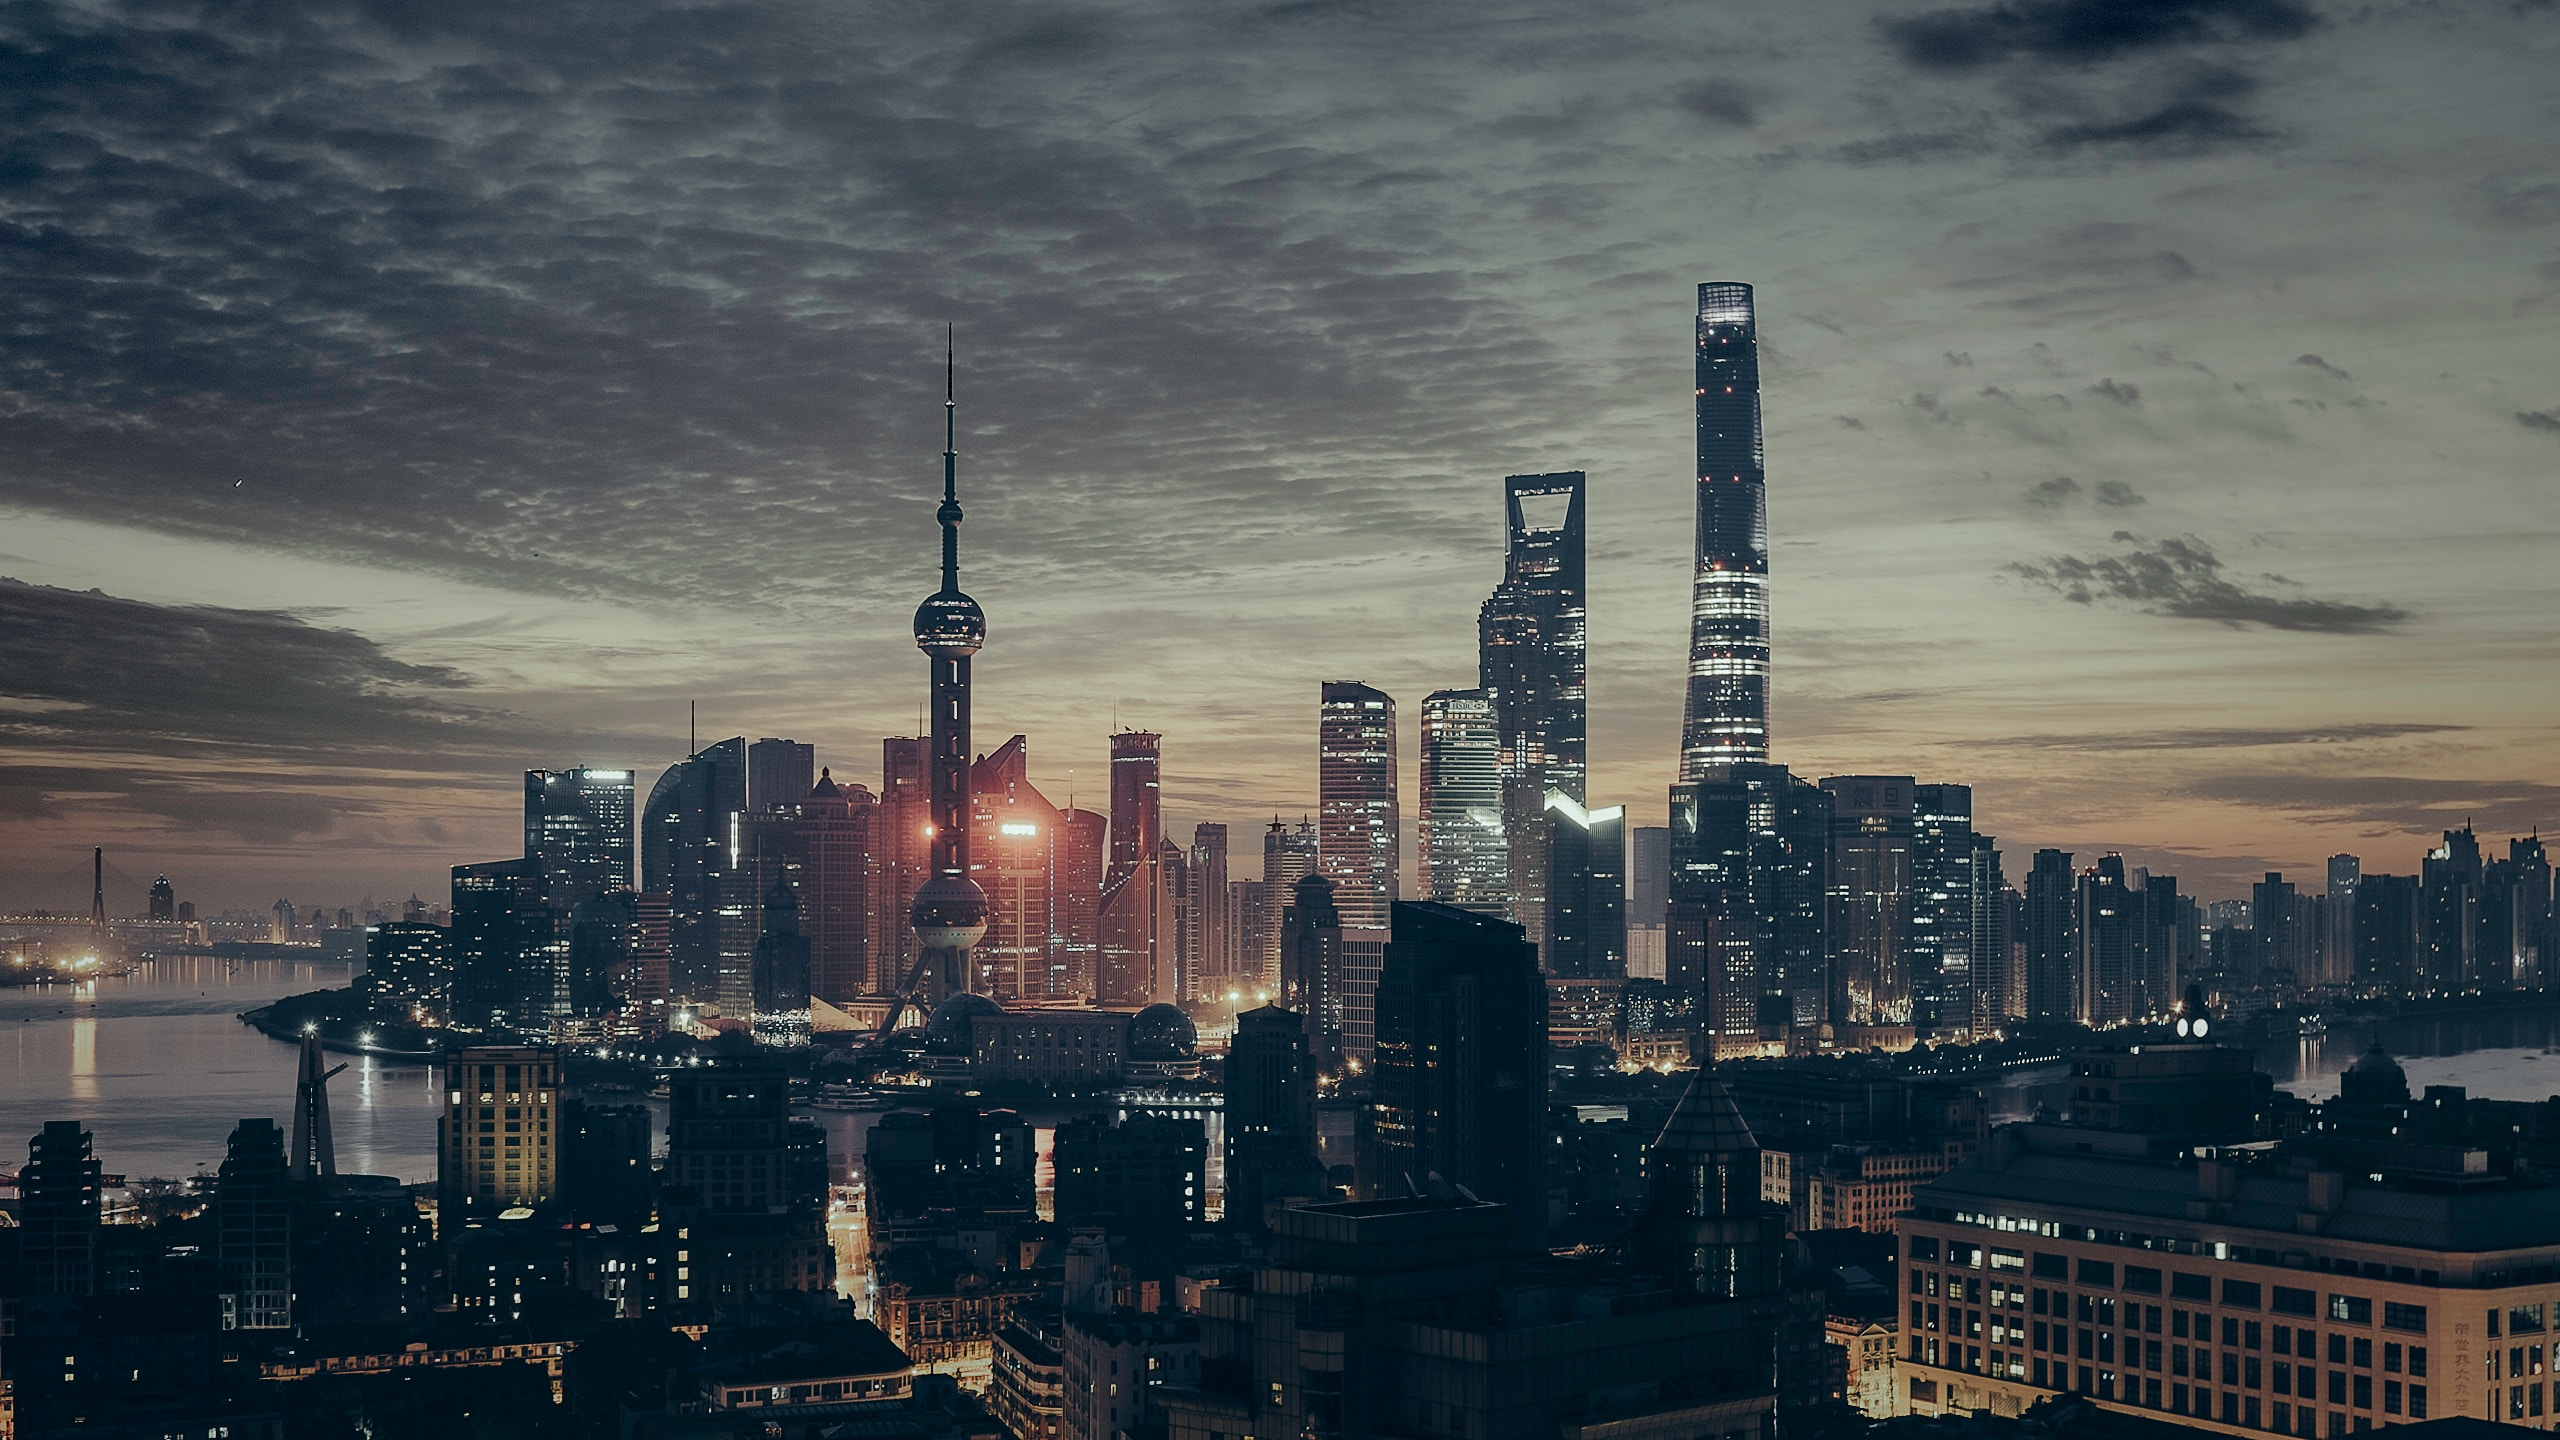
\includegraphics[scale = 0.5]{Img/china-illustration.jpg}
\end{center}
\end{figure}
\author{\Large{Marie \bsc{Chiaverini}} \Large{Baptiste  \bsc{Saclier}} \\\Large{Vadim  \bsc{Crochet}} \Large{Antoine  \bsc{Caillet}} \\\Large{Romain  \bsc{Junca}}}
\date{}
\vfill 
\end{titlepage}
\maketitle
\vspace{5.5cm}
\Large{CESI school of engineers} \hfill \Large{Tutor : Thierry \bsc{BLANC}}
\thispagestyle{empty}
\setcounter{page}{0}
\newpage

\renewcommand{\contentsname}{\Huge{Table of contents}}
\tableofcontents

\newpage
\renewcommand{\listfigurename}{\Huge{List of figures}}
\listoffigures

\newpage

\section{Introduction}


\end{document}

